%%%%%%%%%%%%%%%%%%%%%%%%%%%%%%%%%%%%%%%%%%%%%%%%%%%%%%%%%%%%%%%%%%%%%%%%%%%%%%
\documentclass[12pt,a4paper]{article}

%%%%%%%%%%%%%%%%%%%%%%%%%%%%%%%%%%%%%%%%%%%%%%%%%%%%%%%%%%%%%%%%%%%%%%%%%%%%%%
% Include a few packages

\usepackage{fontspec}
\setmainfont{TeX Gyre Heros}
\usepackage{hyperref}               % Hyperlinks
\usepackage[british]{babel}         % Use British English
\usepackage{graphicx}               % Graphics
\usepackage[svgnames]{xcolor}       % Colours
\usepackage[hmargin=2cm,vmargin=2cm]{geometry} % Sort out the margins
\usepackage{tikz}                   % Graphics primitives
\usepackage{titlesec}               % Fancy section headings
\usepackage{pdfpages}               % Include pages from other PDFs

%%%%%%%%%%%%%%%%%%%%%%%%%%%%%%%%%%%%%%%%%%%%%%%%%%%%%%%%%%%%%%%%%%%%%%%%%%%%%%
% Package settings

% hyperref
\hypersetup{colorlinks=true, allcolors=black, pdftitle={BAMC 2023 Programme}} 

%%%%%%%%%%%%%%%%%%%%%%%%%%%%%%%%%%%%%%%%%%%%%%%%%%%%%%%%%%%%%%%%%%%%%%%%%%%%%%
% Styling

% Colours defined by the University of Bristol brand guidelines
\definecolor{UniversityRed}{RGB}{171, 31, 45}
\definecolor{CoolGrey}{RGB}{227, 230, 229}
\definecolor{BrightAqua}{RGB}{0, 192, 181}
\definecolor{BrightBlue}{RGB}{12, 198, 222}
\definecolor{BrightOrange}{RGB}{238, 114, 25}
\definecolor{BrightPurple}{RGB}{146, 120, 209}
\definecolor{BrightPink}{RGB}{224, 36, 154}
\definecolor{BrightLime}{RGB}{190, 214, 0}
\definecolor{DarkAqua}{RGB}{0, 67, 79}
\definecolor{DarkBlue}{RGB}{0, 47, 95}
\definecolor{DarkOrange}{RGB}{109, 38, 1}
\definecolor{DarkPurple}{RGB}{66, 20, 95}
\definecolor{DarkPink}{RGB}{119, 32, 89}
\definecolor{DarkLime}{RGB}{83, 104, 43}

% Paragraphs are separated by vertical space rather than indents
\setlength{\parindent}{0em}
\setlength{\parskip}{1.5ex plus 0.5ex minus 0.5ex}

% Where to find graphics
\graphicspath{{.}{./images/}}

% Remove section numbers
\setcounter{secnumdepth}{0}

% Format sections and subsections
\titleformat{\section}{\normalfont\LARGE\bfseries\scshape\color{UniversityRed}}{\thesection}{0.2em}{}
\titleformat{\subsection}{\normalfont\large\bfseries\color{DarkBlue}}{\thesubsection}{0.2em}{}
\newcommand{\sectionbreak}{\clearpage}

%\pagestyle{empty}

%%%%%%%%%%%%%%%%%%%%%%%%%%%%%%%%%%%%%%%%%%%%%%%%%%%%%%%%%%%%%%%%%%%%%%%%%%%%%%
% Begin the text

\begin{document}
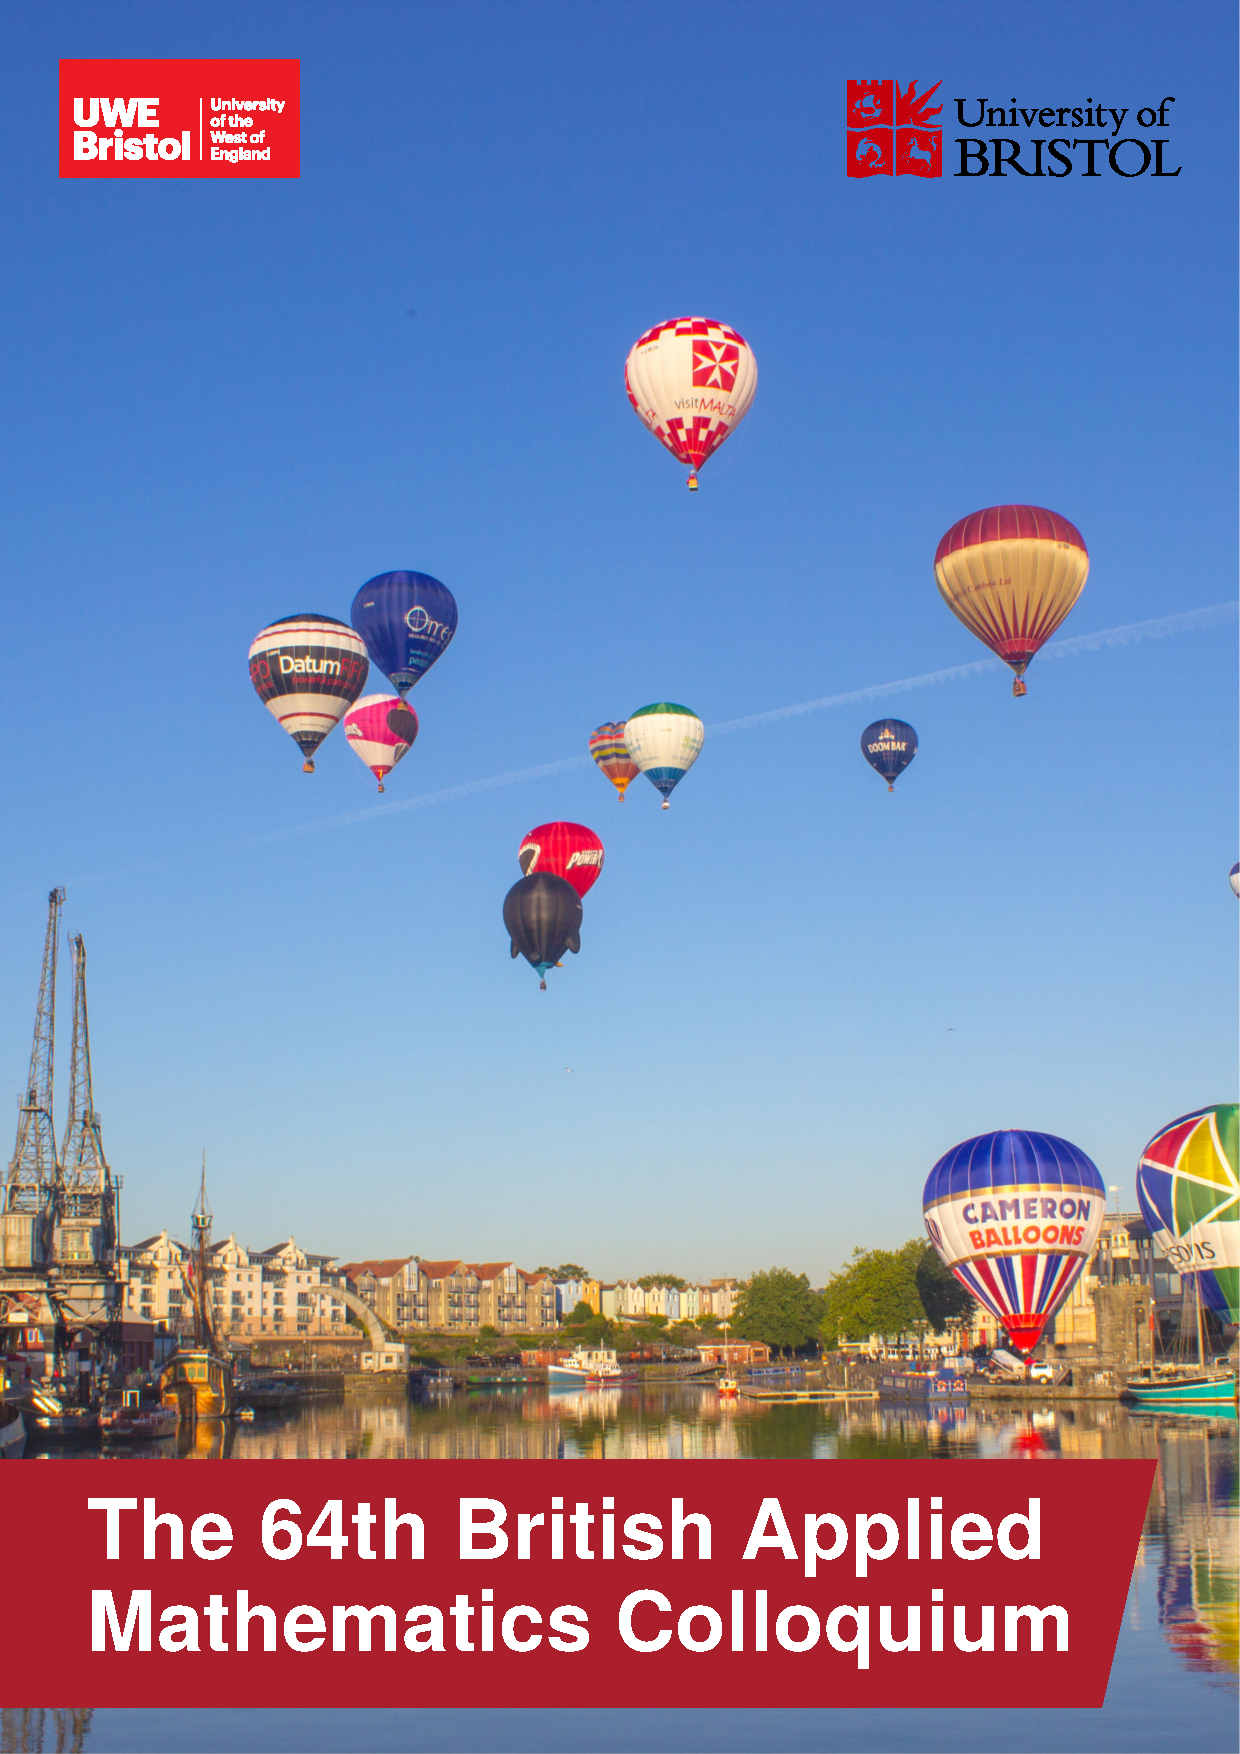
\includepdf{frontpage.pdf}
\setcounter{page}{1}

\section{Welcome}

\textcolor{DarkBlue}{\large Dear participants of the 64th BAMC, welcome to Bristol!}

The BAMC is a meeting that has a central place in the UK Applied Mathematics calendar. It is one of the first places where PhD students and Early Career Researchers present their work, and where mathematicians across all career stages have a chance to actively interact with each other.

\section{Essential Information}

\subsection{Website and latest information}

\subsection{Registration}

\subsection{Refreshments}

\subsection{Monday evening Poster Session and CUP wine reception}

\subsection{Conference Gala Dinner}

\subsection{Bars and pubs}

\subsection{Taxis}

\subsection{Parking on campus}

\subsection{Accommodation}

\subsection{Wi-Fi Access}

\section{Plenary Speakers}

\section{Programme Overview}

\section{Minisymposia Sessions}

\section{Contributed Talks Sessions}

\section{Poster Presentation}

\section{Sponsors, Funders, and Exhibitors}

\section{Map}

\end{document}
